% !TeX root = ../script.tex

\newpage
\section{Stichproben und Stichprobenfunktion}

\begin{colbox}{Definition}[Stichprobe]
    Es sei $X$ eine Zufallsgröße auf einem Wahrscheinlichkeitsraum $(\Omega,\mathcal{F}, \P)$ mit der 
    Verteilungsfunktion $F$. Ein zufälliger Vektor $(X_1,\dots,X_n)^T$ heißt (mathematische) Stichprobe, bzw. unabhängige Beobachtung
    von $X$, falls 
    \begin{enumerate}
        \item $F_{X_1}=\dots=F_{X_n}=F$,
        \item $X_1,\dots,X_n$ sind unabhängig,
    \end{enumerate}
    d.h. $X_1,\dots,X_n$ sind unabhängig und identisch verteilt wie $X$. \\
    Eine Realisierung $(X_1(\omega),\dots,X_n(\omega))^T=(x_1,\dots,x_n)^T$ für ein $\omega\in\Omega$, heißt 
    konkrete Stichprobe / konkrete Beobachtung von $X$.
\end{colbox}

\begin{colbox}{Definition}[Stichprobenfunktion]
    Eine Borel-messbare Abbildung $\phi:\R^n\to\R^m$ heißt Stichprobenfunktion, insbesondere heißt eine 
    Abbildung $\varphi(X_1,\dots,X_n):\Omega\to\R^m$ mit 
    $\varphi(X_1,\dots,X_n)(\omega) = \varphi(X_1(\omega), \dots,X_n(\omega))$ Statistik oder auch zufällige
    Stichprobenfunktion.
\end{colbox}

\begin{colbox}{Definition}[Stichprobenmittel]
    Sei $(X_1,\dots,X_n)$ eine mathematische Stichprobe, dann heißt die Zufallsvariable 
    \[
        \overline{X}_n := \dfrac{1}{n}\sum_{i=1}^{n} X_i
    \]
    Stichprobenmittel bzw. empirischer Erwartungswert. Demnach ist für eine konkrete Stichprobe $(x_1,\dots,x_n)$ der 
    Wert $\overline{x}_n = \tfrac{1}{n}\sum_{i=1}^{n}x_i$ das konkrete Stichprobenmittel.
\end{colbox}

\begin{colbox}{Satz}
    Für das Stichprobenmittel gilt:
    \[
        \E[\overline{X}_n] = \E[X], \qquad D^2[\overline{X}_n] = \dfrac{D^2[X]}{n}
    \]
\end{colbox}
\textit{Beweis.} Beide Gleichungen folgen aus der Linearität von Erwartungswert und Varianz (wegen Unabhängigkeit):
\begin{align*}
    \E[\overline{X}_n] 
    &= \E\left[\dfrac{1}{n}\sum_{i=1}^{n} X_i\right] 
    = \dfrac{1}{n}\cdot\sum_{i=1}^{n}\E[X_i] 
    = \dfrac{1}{n}\cdot n\cdot\E[X]
    = E[X] \\
    D^2[\overline{X}_n] 
    &= D^2\left[\dfrac{1}{n}\sum_{i=1}^{n} X_i\right]
    = \dfrac{1}{n^2}\cdot\sum_{i=1}^{n}D^2[X_i]
    = \dfrac{1}{n^2}\cdot n\cdot D^2[X]
    = \dfrac{D^2[X]}{n}
\end{align*}
\qed

Der empirische Erwartungswert nähert sich dem echten Erwartungswert an, d.h. 
\[
    \E|\overline{X}_n-\E[X]| = \E|\overline{X}_n-\E[\overline{X}_n]| = D^2[\overline{X}_n] = \dfrac{D^2[X]}{n} \nto 0
\]

Tatsächlich nähert sich $\overline{X}_n$ dem Erwartungswert sogar fast sicher an:

\begin{colbox}{Satz}\label{satz:conFSempE}
    Der empirische Erwartungswert konvergiert fast sicher gegen den Erwartungswert, d.h.
    \[
        \P\left(\lim_{n\to\infty}\overline{X}_n = \E[X]\right) = 1
    \]
    Außerdem gilt 
    \[
        \lim_{n\to\infty} \P\left(\sqrt{n}\cdot\dfrac{\overline{X}_n-\E[X]}{\sqrt{D^2[X]}}\leq x\right) = \Phi(x)
    \]
    für jedes $x\in\R$. (Dabei ist $\Phi$ die Verteilungsfunktion der Standardnormalverteilung)
\end{colbox}
\textit{Beweis.}\\
Der erste Teil des Satzes folgt direkt aus dem Gesetz der großen Zahlen. 

Für den zweiten Teil des Satzes verwenden wir den zentralen Grenzwertsatz, denn es gilt $S_n=n\cdot \overline{X}_n$
und damit
\[
    \sqrt{n}\cdot\dfrac{\overline{X}_n-\E[X]}{\sqrt{D^2[X]}}
    = \sqrt{n}\cdot\dfrac{\tfrac{1}{n}(S_n-\E[S_n])}{\sqrt{D^2[X]}}
    = \dfrac{S_n-\E[S_n]}{\sqrt{D^2[S_n]}}
\]
Es folgt
\[
    \P\left(\sqrt{n}\cdot\dfrac{\overline{X}_n-\E[X]}{\sqrt{D^2[X]}}\leq x\right) 
    = \P\left(\dfrac{S_n-\E[S_n]}{\sqrt{D^2[S_n]}}\leq x\right)
    \nto \Phi(x)
\]
\qed

Der zweite Teil des Satzes liefert eine Auskunft über die Abweichung von $\overline{X}_n$ gegenüber $\E[X]$:
\[
    \P(|\overline{X}_n-\E[X]|>\varepsilon) \approx 2-2\Phi\left(\dfrac{\varepsilon \sqrt{n}}{\sqrt{D^2[X]}}\right)
\]

\begin{colbox}{Beispiel}[Schätzen von unbekanntem Parameter]\label{bsp:schaetzungUnPara}
    \begin{enumerate}
        \item[(a)] Eine Versicherung weiß, dass die Anzahl der Schäden $X$ pro Tag poissonverteilt mit Parameter
        $\lambda=\E[X]$ ist. Zwar ist $\lambda$ unbekannt, jedoch kann dieser anhand von Beobachtungen $X_1,\dots,X_n$
        geschätzt werden:
        \[
            \lambda \approx \overline{X}_n = \dfrac{1}{n}\sum_{i=1}^{n} X_i \qquad\text{für } n \text{ groß genug.}
        \]
        \item[(b)] Die Körpergröße $X$ einer zufällig ausgewählten Person in Rostock ist normalverteilt und hat damit 
        die Verteilungsfunktion
        \[
            \Phi(x;\mu,\sigma^2) 
            = \dfrac{1}{\sqrt{2\pi\sigma^2}}
            \cdot\int_{-\infty}^{x}e^{-\tfrac{1}{2}\left(\tfrac{t-\mu}{\sigma}\right)^2}\diff t
        \]
        Um eine vollständige Charakterisierung zu tätigen, benötigen wir noch Schätzwerte für die Parameter 
        $\mu$ und $\sigma^2$ durch 
        \[
            \mu = \E[X] \approx \dfrac{1}{n}\sum_{i=1}^{n} X_i
        \]
        \item[(c)] Ein Supermarkt weiß, dass die Zeit $X$ bis zur Ankunft eines neuen Kunden an der Supermarktkasse 
        exponentialverteilt mit Parameter $\lambda$ ist. Die Wartezeiten werden $n$ mal beobachtet, so dass 
        \[
            \lambda = \dfrac{1}{\E[X]} \approx \dfrac{n}{\sum_{i=1}^{n} X_i}
        \]
    \end{enumerate}
\end{colbox}

Für die Charakterisierung einiger Verteilungen benötigen wir neben dem Erwartungswert auch noch eine Schätzung für 
die Varianz $D^2[X]$.

Wir betrachten hierfür eine weitere Stichprobenfunktion:

\begin{colbox}{Definition}[Stichprobenvarianz]
    Sei $X_1,\dots,X_n$ eine mathematische Stichprobe, dann heißt die Zufallsgröße
    \[
        S_n^2 = \dfrac{1}{n-1} \sum_{i=1}^{n} (X_i-\overline{X}_n)^2
    \]
    Stichprobenvarianz bzw. empirische Varianz. Für eine konkrete Stichprobe $x_1,\dots,x_n$ ist demnach
    $s_n^2 = \tfrac{1}{n-1} \sum_{i=1}^{n} (X_i-\overline{X}_n)^2$ die konkrete Stichprobenvarianz.
\end{colbox}

\begin{colbox}{Satz}\label{satz:conFSempV}
    Für die Stichprobenvarianz gilt 
    \[
        \E[S_n^2] = D^2[X]
    \]
    Existiert zusätzlich das 4. Moment von $X$, d.h. $\E X^4<\infty$, so ergibt sich 
    \[
        D^2[S_n^2] = \dfrac{1}{n}\left(\E(X-\E[X])^4-\dfrac{n-3}{n-1}(D^2[X])\right)
    \]
\end{colbox}
\textit{Beweis.} \\
Der erste Teil des Satzes ergibt mit dem Ansatz
\[
    S_n^2 
    = \dfrac{1}{n-1} \sum_{i=1}^{n} (X_i-\overline{X}_n)^2 
    = \dfrac{1}{n-1} \sum_{i=1}^{n} \left((X_i-\E[X]) - \dfrac{1}{n}\sum_{j=1}^{n}(X_j-\E[X])\right)^2
\]
Da der Erwartungswert von $X_i-\E[X]$ durch $0$ gegeben ist, lässt sich ab nun o.B.d.A. annehmen, dass $\E[X]=0$ gilt.
Es ergibt sich die Umformung zu 
\[
    S_n^2 
    = \dfrac{1}{n-1} \sum_{i=1}^{n}(X_i-\overline{X}_n)^2 
    = \dfrac{1}{n-1} \sum_{i=1}^{n}(X_i^2-2X_i\overline{X}_n+\overline{X}_n^2)
    = \dfrac{1}{n-1} \left(\sum_{i=1}^{n} X_i^2 - n\cdot\overline{X}_n^2\right)
\] 
und damit für den Erwartungswert
\[
    \E[S_n^2] 
    = \dfrac{1}{n-1} \left(\sum_{i=1}^{n} \E[X_i^2] - n\cdot\E[\overline{X}_n^2]\right)
    =\dfrac{1}{n-1} \left(\sum_{i=1}^{n} D^2[X] - D^2[X]\right) 
    = D^2[X]
\] 

Der zweite Teil des Satzes sei ausgelassen.
\qed

Der Satz garantiert die Konvergenz im quadratischen Mittel. Auch hier lässt sicher zusätzlich noch fast sichere 
Konvergenz folgern:

\begin{colbox}{Satz}
    Die empirische Varianz konvergiert fast sicher gegen die Varianz, d.h. 
    \[
        \P\left(\lim_{n\to\infty} S_n^2 = D^2[X]\right) = 1
    \]
    Falls $\E[X^4] < \infty$ so gilt weiter 
    \[
        \lim_{n\to\infty} \P\left(\sqrt{n}\cdot\frac{S_n^2 - D^2[X]}{\sqrt{\E(X-\E[X])^4 - (D^2[X])^2}} \leq x\right) 
        = \Phi(x)
    \]
\end{colbox}
\textit{Beweis.} Aus der Unabhängigkeit von $X_1,\dots,X_n$ folgt auch die von $X_1^2,\dots,X_n^2$ und somit liefert
das Gesetz der großen Zahlen, dass $\tfrac{1}{n}\sum_{i=1}^{n} X_i^2 \conFS \E[X^2]$ und nach aus 
Satz \ref{satz:conFSempE} folgt zusätzlich $\overline{X}_n^2 \conFS (\E[X])^2$.

Analog zum Beweis von Satz \ref{satz:conFSempV} ergibt sich damit 
\[
    S_n^2 
    = \dfrac{1}{n-1}\left(\sum_{i=1}^{n}X_i^2 - n\cdot \overline{X}_n^2\right) 
    = \dfrac{n}{n-1}\left(\dfrac{1}{n}\sum_{i=1}^{n}X_i^2 - \overline{X}_n^2\right) 
    \nto 1\cdot(\E[X^2] - (E[X])^2) = D^2[X]
\]
Der zweite Teil sei erneut ohne Beweis.
\qed 

\begin{colbox}{Beispiel}[Weiterführung von Beispiel \ref{bsp:schaetzungUnPara}]
    Wir sind nun in der Lage für eine Normalverteilung den zweiten Parameter $\sigma^2$ zu schätzen:
    \[
        \sigma^2 = D^2[X] \approx\dfrac{1}{n-1}\sum_{i=1}^{n}(X_i-\overline{X}_n)^2
    \]
\end{colbox}

\begin{colbox}{Satz}
    Für den empirischen Erwartungswert und Varianz ergibt sich folgende verwandte Form des zentralen Grenzwertsatzes:
    \[
        \lim_{n\to\infty} \P\left(\sqrt{n}\cdot\dfrac{\overline{X}_n-\E[X]}{\sqrt{S_n^2}}\leq x\right) = \Phi(x)
    \]
\end{colbox}
\textit{Beweis.} Die Konvergenz folgt direkt aus dem zentralen Grenzwertsatz, denn 
\begin{align*}
    \sqrt{n}\cdot\dfrac{\overline{X}_n-\E[X]}{\sqrt{S_n^2}} 
    &= \sqrt{n}\cdot\dfrac{\overline{X}_n-\E[X]}{\sqrt{D^2[X]}} \cdot \dfrac{\sqrt{D^2[X]}}{\sqrt{S_n^2}}
    = \sqrt{n}\cdot\dfrac{\tfrac{1}{n}S_n-\tfrac{1}{n}\E[S_n]}{\tfrac{1}{n}\sqrt{D^2[S_n]}} \cdot \sqrt{\dfrac{D^2[X]}{S_n^2}}\\
    &= \dfrac{S_n-\E[S_n]}{\sqrt{D^2[S_n]}} \cdot \underbrace{\sqrt{\dfrac{D^2[X]}{S_n^2}}}_{\conD 1}
    \conD Z\sim\mathcal{N}(0,1)
\end{align*}

\begin{colbox}{Bemerkung}
    Dieser Satz ermöglicht es sogenannte Konfidenzintervalle (später mehr) anzugeben, d.h. einen Bereich für 
    welchen die Wahrscheinlichkeit, dass $|\overline{X}_n-\E[X]|$ darin liegt, einen festen Wert annimmt. 
    Sei hierfür $z_\alpha\in(0,1)$ das $\alpha$-Quantil der Standardnormalverteilung, d.h. $\Phi(z_\alpha)=\alpha$, 
    dann gilt 
    \[
        \P\left(|\overline{X}_n-\E[X]|<\dfrac{z_{1-\alpha\,/\,2}S_n}{\sqrt{n}}\right) \approx 1-\alpha
    \] 
\end{colbox}

\begin{colbox}{Satz}
    Für eine mathematische Stichprobe $X_1,\dots,X_n$ von $X\sim\mathcal{N}(\mu,\sigma^2)$ sind $\overline{X}_n$ und 
    $S_n^2$ unabhängige Zufallsgrößen und es gilt
    \[
        \overline{X}_n\sim\mathcal{N}(\mu,\tfrac{\sigma^2}{n}), \quad
        \dfrac{(n-1)S_n^2}{\sigma^2}\sim\chi^2_{n-1}, \quad
        \dfrac{\sqrt{n}(\overline{X}_n-\mu)}{S_n}\sim t_{n-1}
    \]
\end{colbox}
\textit{Beweis.} Ohne Beweis.

\begin{colbox}{Bemerkung}
    \begin{enumerate}
        \item $\chi_n^2$ ist die Chi-Quadrat Verteilung, sie ist die Summe von $n$ unabhängigen
        quadratischen Standardnormalverteilung, d.h. 
        \[X_1,\dots,X_n\sim\mathcal{N}(0,1) \implies \sum_{i=1}^{n} X_i^2\sim\chi^2_n\]
        Sie hat folgende Dichtefunktion:
        \[
            f_{\chi_n^2}(x) = \dfrac{x^{k/2-1}e^{-k/2}}{2^{k/2}\Gamma(\tfrac{k}{2})}\One_{(0,\infty)}
        \]
        \item $t_n$ ist die studentsche t-Verteilung. Für Zufallsgrößen $X\sim\mathcal{N}(0,1)$ und $U_n\sim\chi^2_n$ 
        gilt 
        \[
            \dfrac{X}{\sqrt{\tfrac{U_n}{n}}} \sim t_n
        \]
        Die Dichte ist gegeben durch
        \[
            f_{t_n} = \dfrac{\Gamma\left(\frac{n+1}{2}\right)}{\sqrt{n\pi}\,\Gamma\left(\frac{n}{2}\right)} 
            \left(1+\frac{x^2}{n}\right)^{-\frac{n+1}{2}}
        \]
    \end{enumerate}
\end{colbox}

\begin{colbox}{Beispiel}[Schätzer einer Einzelwahrscheinlichkeit]
    Gegeben seien $(X_n)$ unabhängig und Bernoulliverteilt mit Parameter $p=\P(A)$ für ein Ereignis $A$, d.h. 
    \[
        \P(X_n=1) = p,\quad \P(X_n=0) = 1-p
    \]
    Für Ergebnisse $\omega=(\omega_1,\omega_2,\dots)$ gilt
    \[
        X_n(\omega) = 1_\{A\}(\omega_n) = \begin{cases}
            1 & \omega_n \in A \\
            0 & \omega_n \notin A \\
        \end{cases}
    \]
    dabei bedeutet $\omega_n\in A$, dass das Ereignis $A$ in der $n$-ten Wiederholung des Experiments eintrifft. 

    Die absolute Häufigkeit $H_n(A) = \sum_{k=1}^{n} X_k$ beschreibt wie oft das Ereignis $A$ in den ersten $n$ 
    Versuchen eintrifft, die relative Häufigkeit ist gegeben durch $h_n(A) = \tfrac{H_n(A)}{n}$ und es gilt 
    \[
        h_n(A) = \dfrac{1}{n}\sum_{k=1}^{n} X_k \conFS \E[X] = \P(A)
    \]
\end{colbox}

\begin{colbox}{Beispiel}
    5 Mal wird der zufällige Versuch Würfeln $n$-fach wiederholt. Sei zudem $A = \{1,2\}$. 
    Wir würfeln am Computer für verschiedene $n$:
\begin{table}[ht]
  \centering
  \begin{tabular}{c|ccccc}
    \toprule
    \(n\) & \multicolumn{5}{c}{\(h_n(A)\)} \\
    \midrule
    6             & \(\tfrac{3}{6}\)   & \(\tfrac{5}{6}\)   & \(\tfrac{2}{6}\)   & \(\tfrac{3}{6}\)   & \(\tfrac{2}{6}\)   \\
    \(6\cdot10^3\) & 0.34567            & 0.33017            & 0.32800            & 0.33033            & 0.33067            \\
    \(6\cdot10^6\) & 0.33325            & 0.33311            & 0.33346            & 0.33330            & 0.33319            \\
    \bottomrule
  \end{tabular}
\end{table}
\end{colbox}

Ein intuitiver Schätzer der Varianz ergibt sich aus
\[
    \tilde{S}_n^2 = \dfrac{1}{n} \sum_{i=1}^{n} (X_i - \overline{X}_j)^2
\]
Auch für diesen Schätzer gilt $\tilde{S}_n^2 \conFS D^2[X]$, da $\tilde{S}_n^2=\tfrac{n-1}{n}S_b^2$. Es gilt jedoch 
\[
    \E[\tilde{S}_n^2] = \dfrac{n-1}{n}\E[S_n^2] = \dfrac{n-1}{n}D^2[X] < D^2[X]
\]

Für den Fall das der echte Wert von $\E[X]$ bekannt ist, funktioniert dieser Ansatz, denn für 
\[
    \hat{S}_n^2 = \dfrac{1}{n} \sum_{i=1}^{n} (X_i - \E[X])^2
\]

ergibt sich 
\begin{align*}
    \E[\hat{S}_n^2] 
    &= \dfrac{1}{n} \sum_{i=1}^{n} \E(X_i - \E[X])^2 
    = \dfrac{1}{n} \left(\sum_{i=1}^{n} \E[X_i^2] - 2\E[X]\sum_{i=1}^{n} \E[X_i] + n(\E[X])^2 \right) \\
    &= \E[X^2] - 2(\E[X])^2 + (\E[X])^2 
    = D^2[X] \\
    \hat{S}_n^2 &= \dfrac{1}{n}\sum_{i=1}^{n}X_i^2 - 2\E[X]\cdot\dfrac{1}{n}\sum_{i=1}^{n}X_i + (\E[X])^2 \conFS D^2[X]
\end{align*}

\begin{colbox}{Definition}[Momentschätzer]
    Sei $X_1,\dots,X_n$ eine Stichprobe einer Zufallsgröße $X$ mit $\E|X|^k < \infty$. 
    \begin{enumerate}
        \item Das $k$-te Moment $\E[X^k]$ kann durch 
        \[
            \hat{m}_k = \dfrac{1}{n}\sum_{i=1}^{n} X_i^k
        \]
        geschätzt werden. Dieser Schätzer ist erwartungstreu, d.h. $\E[\hat{m}_k]=\E[X^k]$, und konvergiert fast sicher 
        gegen das $k$-te Moment.
        \item Das $k$-te zentrierte Moment $\E(X-\E[X])^k$ kann durch 
        \[
            \hat{\mu}_k = \dfrac{1}{n-1}\sum_{i=1}^{n}(X_i-\overline{X}_n)^k
        \]
        geschätzt werden. Auch dieser Schätzer ist erwartungstreu und konvergiert fast sicher.
    \end{enumerate}
    Sei $(X_1,Y_1), \dots, (X_n,Y_n)$ eine Stichprobe eines Zufallsvektors $(X,Y)$ mit $D^2[X],D^2[Y]<\infty$, so ist 
    \[
        \hat{C}_{X,Y} = \dfrac{1}{n-1}\sum_{i=1}^{n}(X_i-\overline{X}_n)(Y_i-\overline{Y}_n)
    \]
    die empirische Kovarianz, ein Schätzer für $\mathrm{cov}(X,Y)$. Der Korrelationskoeffizient wird demnach durch
    den empirischen Korrelationskoeffizient 
    \[
        \hat{\rho}_{XY} 
        = \dfrac{\sum_{i=1}^{n}(X_i-\overline{X}_n)(Y_i-\overline{Y}_n)}
        {\sqrt{\sum_{i=1}^{n}(X_i-\overline{X}_n)^2}\sqrt{\sum_{i=1}^{n}(Y_i-\overline{Y}_n)^2}}
    \]
    der Korrelationskoeffizient geschätzt.
\end{colbox}

\begin{colbox}{Beispiel}[Empirischer Korrelationskoeffizient]
    Nun steht $X$ für die Note eines zufällig ausgewählten Schülers in Mathematik und $Y$ für dessen Note in Physik. 
    Lehrer fragen sich, wie groß der Zusammenhang zwischen $X$ und $Y$ ist und nehmen eine 
    konkrete Stichprobe $(x_1, y_1), (x_2, y_2), \dots, (x_{10}, y_{10})$:

    \begin{center}
    \begin{tabular}{c|cccccccccc}
        $i$   & 1 & 2 & 3 & 4 & 5 & 6 & 7 & 8 & 9 & 10 \\
        \hline
        $x_i$ & 1 & 3 & 2 & 1 & 5 & 2 & 3 & 4 & 4 & 3 \\
        $y_i$ & 1 & 3 & 1 & 3 & 4 & 2 & 3 & 3 & 5 & 3 \\
    \end{tabular}
    \end{center}

    Das arithmetische Mittel beträgt $\overline{x}_n = \overline{y}_n = 2.8$.

    Der empirische Korrelationskoeffizient berechnet sich zu
    \[
        \hat{\rho}_{XY} = 
        \frac{(1-2.8)(1-2.8) + (3-2.8)(3-2.8) + (2-2.8)(1-2.8) + \dots}
        {\sqrt{(1-2.8)^2 + (3-2.8)^2 + \dots}\sqrt{(1-2.8)^2 + (3-2.8)^2 + \dots}}
        = 0.73
    \]
    Da die Schätzung nahe $1$ liegt, scheint ein großer Zusammenhang zwischen Mathe- und Physiknoten zu bestehen.
\end{colbox}

\begin{colbox}{Bemerkung}[Schätzer, als Integralnäherung]
    Sei $g:[a,b]\to\R$ eine stetige Funktion, gesucht ist der Wert des Integrals $\int_{a}^{b} g(x)\diff x$.

    Durch die Verwendung einer auf $[a,b]$ gleichverteilten Zufallsgröße $X$ ergibt sich 
    \[
        \int_{a}^{b} g(x)\diff x = (b-a)\cdot\int_{a}^{b}f_X(x)g(x)\diff x = (b-a)\E[g(X)]
    \]
    Sei nun $X_1,\dots,X_n$ eine Stichprobe von $X$, so gilt 
    \[
        \dfrac{1}{n}\sum_{i=1}^{n} g(X_i) \conFS \E[g(X)],
        \quad \text{d.h.}\quad
        \int_{a}^{b} g(x)\diff x \approx (b-a)\cdot \dfrac{1}{n}\sum_{i=1}^{n} g(X_i)
    \]
    Solche auf $[a,b]$ generierten gleichverteilten Zufallszahlen (z.B. am Rechner) 
    ermöglichen demnach eine (Monte-Carlo) Approximation des Integrals.
\end{colbox}

\begin{colbox}{Definition}[Ordnungsstatistik]
    Sei $X_1,\dots,X_n$ eine Stichprobe und 
    \[
        \phi(x_1,\dots,x_n) = (x_{(1)}, \dots,x_{(n)}) 
        \qquad \text{mit } x_{(i)} = \min\big\{x_j\,:\,\#\{k:x_k\leq x_j\} \geq i\big\}
    \]
    die Permutation, welche $x_1,\dots,x_n$ der Größe nach ordnen, d.h. $x_{(1)}\leq\dots\leq x_{(n)}$.

    Die Zufallsvariablen $X_{(1)},\dots,X_{(n)}$, gegeben durch 
    \[
        (X_{(1)}(\omega),\dots,X_{(n)}(\omega)) = \phi(X_1(\omega),\dots,X_n(\omega)), \quad\forall\omega\in\Omega
    \]
\end{colbox}

\begin{colbox}{Definition}
    Für eine Ordnungsstatistik $X_{(1)},\dots,X_{(n)}$ sei $R_n := X_{(n)}-X_{(1)}$ die Stichprobenspannweite und 
    \[
        M_n := \begin{cases}
            X_{(\tfrac{n+1}{2})}, & n \text{ ungerade} \\
            \tfrac{1}{2}X_{(\tfrac{n}{2})}+\tfrac{1}{2}X_{(\tfrac{n}{2}+1)}, & n \text{ gerade}
        \end{cases}
    \]
    der Stichprobenmedian.
\end{colbox}

Der Stichprobenmedian dient als alternative zum klassischen Mittelwert. Etwa die Hälfte der Stichprobe liegt unter 
$M_n$ und hat den Vorteil, dass extremale Werte bei $X_{(1)}$ oder $X_{(n)}$ ihn weniger verzerren, als es 
bei $\overline{X}_n$ passieren würde.

\begin{colbox}{Satz}
    Sei $X_1,\dots,X_n$ eine Stichprobe zu einer diskreten Zufallsgröße $X$ mit aufsteigendem Wertebereich 
    $x_0 < \dots < x_m$ für $m\in\N\cup\{\infty\}$, so gilt
    \[
        \P(X_{(i)}\leq x_j) = \sum_{k=i}^{n} \binom{n}{n} P_j^k\cdot (1-P_j)^{n-k}
    \]
    wobei $P_j = \P(X\leq x_j) = \sum_{k=0}^{j} \P(X=x_k)$.
\end{colbox}
\textit{Beweis.} Die Ereignisse $\{X\leq x_j\}$ und $\{X > x_j\}$ beschreiben Erfolg und Misserfolg eines 
bernoulliverteiltem Ereignis mit Erfolgswahrscheinlichkeit $P_j$. 
Damit $X_{(i)}\leq x_j$ muss dieses Ereignis mindestens $i$ Mal eintreffen. Dabei ist das Eintreffen von $k$-fachem 
Erfolg binomialverteilt. 

\begin{colbox}{Satz}
    Sei $X_1,\dots,X_n$ eine Stichprobe zu einer Zufallsgröße mit Dichtefunktion $f$ und zugehöriger Verteilungsfunktion
    $F(x)=\int_{-\infty}^{x}f(y)\diff y$, dann ist die Dichte der Ordnungsstatistik $X_{(i)}$ gegeben durch 
    \[
        f_{X_{(i)}}(x) = \binom{n}{i} \cdot i\cdot f(x)\cdot F(x)^{i-1}\cdot F(x)^{n-i}
    \]
\end{colbox}
\textit{ohne Beweis.}

\begin{colbox}{Beispiel}
    Seien die Stichprobenvariablen $X_1,\dots,X_n$ gleichverteilt auf dem Intervall $[0,b]$. Dann haben diese
    die folgende Dichte- und Verteilungsfunktion
    \[
        f(x) = \dfrac{1}{b}\cdot\One_{[0,b]}(x), \qquad F(x)=\begin{cases}
            0, &x<0 \\
            \tfrac{x}{b}, &x\in[0,b]\\
            1, &x>1
        \end{cases}
    \]
    Für die Ordnungsstatistik ergibt sich:
    \[
        f_{X_{(i)}}(x) = \dfrac{n!}{(i-1)!(n-i)!}\cdot\dfrac{x^{i-1}}{b^n}\cdot(b-x)^{n-1}\cdot\One_{[0,b]}(x)
    \]
    und es folgt
    \begin{align*}
        \E[X_{(i)}] 
        &= \int_{0}^{b} \dfrac{n!}{(i-1)!(n-i)!}\cdot\dfrac{x^{i}}{b^n}\cdot(b-x)^{n-1} \diff x 
        = \dfrac{ib}{n+1} \\
        D^2[X_{(i)}] &= \dots = \dfrac{i(n-i+1)b^2}{(n+1)^2(n+2)}
    \end{align*}
\end{colbox}

\begin{colbox}{Definition}
    Sei $X_1,\dots,X_n$ eine Stichprobe der Zufallsgröße $X$, dann ist
    \[
        W_n(x) = \dfrac{1}{n}|\{X_i\,:\,X_i\leq x\}|
    \]
    die empirische Verteilungsfunktion von $X$.
\end{colbox}

Diese Definition gibt die relative Häufigkeit des Ereignis $\{X\leq x\}$ an und liefert damit 
\[
    W_n(x)\approx \P(\{X\leq x\}) = F_X(x)
\]

\begin{colbox}{Satz}[Hauptsatz der Statistik]
    Sei $W_n$ die empirische Verteilung einer Stichprobe $X_1,\dots,X_n$ der Zufallsgröße $X$ mit 
    Verteilungsfunktion $F$, dann gilt für alle $x\in\R$:
    \begin{enumerate}
        \item Die Zufallsgröße $nW_n(x)$ ist binomialverteilt mit Parametern $n$ und $p=F(x)$, d.h.
        \[
            \P(nW_n(x)=k) = \binom{n}{k}\cdot F(x)^k\cdot (1-F(x))^{n-k} \quad \text{für alle } k=0,1,\dots,n
        \]
        \item $\E[W_n(x)] = F(x)$
        \item $D^2[W_n(x)] = \tfrac{1}{n}F(x)(1-F(x))$
        \item $W_n(x)\conFS F(x)$
        \item Falls $0<F(x)<1$, so gilt 
        \[
            \lim_{n\to\infty} \P\left(\sqrt{n}\dfrac{W_n(x)-F(x)}{\sqrt{F(x)(1-F(x))}}\leq y\right) = \Phi(y)
        \]
    \end{enumerate}
\end{colbox}
\textit{Beweis.}
\begin{enumerate}
    \item Für $p=F(x)$ sei $Y_i(x)$ definiert als 
    \[
        Y_i(x) = \begin{cases}
            1, & X_i \leq x, \text{ mit Wkt. } p \\
            0, & X_i > x, \text{ mit Wkt. } 1-p \\
        \end{cases}
    \]
    dann sind $Y_1(x),\dots,Y_n(x)$ unabhängig und Bernoulliverteilt mit 
    \[
        n\cdot W_n(x) = |\{X_i\leq x\}| = \sum_{i=1}^{n} Y_i(x)\sim\mathrm{Bin}(n,p)
    \]
    \item Mit $Y_i(x)$ aus Teil 1 folgt
    \[
        \E[W_n(x)] = \dfrac{1}{n}\sum_{i=1}^{n}\E[Y_i(x)] = \dfrac{1}{n}\cdot np = p = F(x)
    \]
    \item Analog zu 2. folgt 
    \[
        D^2[W_n(x)] = \dfrac{1}{n^2}\sum_{i=1}^{n}D^2[Y_i(x)] = \dfrac{1}{n^2}\cdot np(1-p) = \dfrac{1}{n}F(x)(1-F(x))
    \]
    \item Nach dem Gesetz der großen Zahlen gilt
    \[
        W_n(X) = \dfrac{1}{n}\sum_{i=1}^{n} Y_i \conFS \E[Y_1(x)] = p = F(x)
    \]
    \item Nach dem zentralen Grenzwertsatz folgt mit $W_n(x)=\tfrac{1}{n}S_n(x)$, dass 
    \begin{align*}
        \sqrt{n}\dfrac{W_n(x)-F(x)}{\sqrt{F(x)(1-F(x))}} 
        &= \sqrt{n}\dfrac{W_n(x)-\E[W_n(x)]}{\sqrt{n\cdot D^2[W_n(x)]}} 
        = \sqrt{n}\dfrac{\tfrac{1}{n}S_n(x)-\tfrac{1}{n}\E[S_n(x)]}{\sqrt{\tfrac{1}{n}D^2[S_n(x)]}}\\
        &= \dfrac{S_n(x)-\E[S_n(x)]}{\sqrt{D^2[S_n(x)]}} 
        \conD Z\sim\mathcal{N}(0,1)
    \end{align*}
\end{enumerate}

Die zweite und dritte Aussage des Satzes garantiert uns, dass $W_n(x)$ ein geeigneter Schätzer ist
(d.h. erwartungstreu und Quadratmittelfehler geht gegen Null).
Die fünfte Aussage erlaubt uns erneut die Bestimmung eines Konfidenzintervalls:
\[
    \P(|W_n(x)-F(x)|>\varepsilon) \approx 2-2\Phi\left(\dfrac{\varepsilon\sqrt{n}}{\sqrt{F(x)(1-F(x))}}\right)
\]

\begin{colbox}{Satz}[Satz von Gliwenko-Cantelli]
    Die Folge $(W_n)$ der empirischen Verteilungsfunktionen konvergiert fast sicher gleichmäßig in $x$, d.h. 
    \[
        \P\left(\sup_{x\in\R}|W_n(x)-F(x)|\nto 0\right) = 1
    \]
\end{colbox}
\textit{ohne Beweis.}

\begin{colbox}{Beispiel}[Empirische Verteilungsfunktion]
    Eine Maschine produziert Teile, die eine gewisse Länge haben sollen. Jedoch weicht die Länge bei der Produktion immer leicht ab. Dieser Fehler ist eine Zufallsgröße $X$ (Abweichung in mm). Konkrete Messungen $x_1, x_2, \dots, x_{50}$ der Abweichungen sehen wie folgt aus:

    \begin{center}
    \begin{tabular}{|c|c|c|c|c|c|}
        \hline
        0.46 & 0.47 & 2.46 & -0.32 & -0.07 \\
        \hline
        0.06 & \textbf{-2.52} & -0.53 & -0.19 & 0.54 \\
        \hline
        1.49 & -0.35 & -0.63 & 0.70 & 0.93 \\
        \hline
        1.02 & -0.47 & 1.28 & \textbf{3.56} & 0.57 \\
        \hline
        1.39 & -0.65 & 0.05 & 0.32 & 2.95 \\
        \hline
        0.30 & -0.29 & 1.30 & 0.24 & -0.96 \\
        \hline
        -1.56 & 0.19 & -1.29 & 0.02 & 0.53 \\
        \hline
        1.38 & 0.79 & -0.96 & -0.85 & -1.87 \\
        \hline
        -1.58 & 0.19 & 1.19 & -0.50 & -0.27 \\
        \hline
        1.97 & -0.26 & 0.41 & 0.44 & -0.04 \\
        \hline
    \end{tabular}
    \end{center}

    Wir interpretieren $X$ als stetige Zufallsgröße und unterteilen die Daten in Klassen. 
    Die empirische Verteilungsfunktion $W_n(x)$ gibt für jedes $x$ die relative Häufigkeit der Werte $x_i \leq x$ 
    an und schätzt damit die Verteilungsfunktion $F_X(x)$.

    Als Faustregel für die Anzahl der Klassen $K$ gilt: 
    \[
        K \leq \log_{10}(n)\cdot 5
    \]
    mit $n=50$ die Klassenanzahl ergibt sich $K=8$. Die Klassen sind:
    \[
        [a_0, a_1), [a_1, a_2), \dots, [a_7, a_8]
    \]
    mit $a_0 = x_{\min} = -2.52$, $a_8 = x_{\max} = 3.56$, sowie 
    
    \[
        a_i = a_0 + i\cdot d, \qquad \text{mit } d = \frac{x_{\max} - x_{\min}}{K} = \frac{6.08}{8} = 0.76
    \]

    Für jede Klasse $[a_i, a_{i+1})$ bestimmen wir die relative Häufigkeit
    \[
        h_n^{(i)} = \frac{1}{n} \cdot \text{Anzahl der } x_j \text{ mit } x_j \in [a_i, a_{i+1})
    \]
    und schätzen damit die Dichte in diesem Intervall durch
    \[
        \P(X\in[a_i,a_{i+1})) = \int_{a_i}^{a_{i+1}} f_X(x)\diff x = f_i\cdot d
    \]
    Das heißt $f_i = \tfrac{h_n^{(i)}}{d}$ ist eine Approximation der Dichte, genannt empirische Dichte. 

    Unsere Werte ergeben:
    \begin{table}[ht]
    \centering
    \begin{tabular}{c l c c c}
    \toprule
    $i$ & Klasse & Klassenhäufigkeit & rel.\ Klassenhäufigkeit $h_n^{(i)}$ & $f_i = \dfrac{h_n^{(i)}}{d}$ \\
    \midrule
    0 & $[-2.52,\,-1.76)$ &  3 & 0.06 & $\approx 0.079$ \\
    1 & $[-1.76,\,-1.00)$ &  2 & 0.04 & $\approx 0.053$ \\
    2 & $[-1.00,\,-0.24)$ & 13 & 0.26 & $\approx 0.342$ \\
    3 & $[-0.24,\,+0.52)$ & 13 & 0.26 & $\approx 0.342$ \\
    4 & $[+0.52,\,+1.28)$ & 10 & 0.20 & $\approx 0.263$ \\
    5 & $[+1.28,\,+2.04)$ &  6 & 0.12 & $\approx 0.158$ \\
    6 & $[+2.04,\,+2.80)$ &  1 & 0.02 & $\approx 0.026$ \\
    7 & $[+2.80,\,+3.56]$ &  2 & 0.04 & $\approx 0.053$ \\
    \bottomrule
    \end{tabular}
    \end{table}

    Die empirische Dichte lässt sich wie folgt skizzieren:
    \begin{center}
        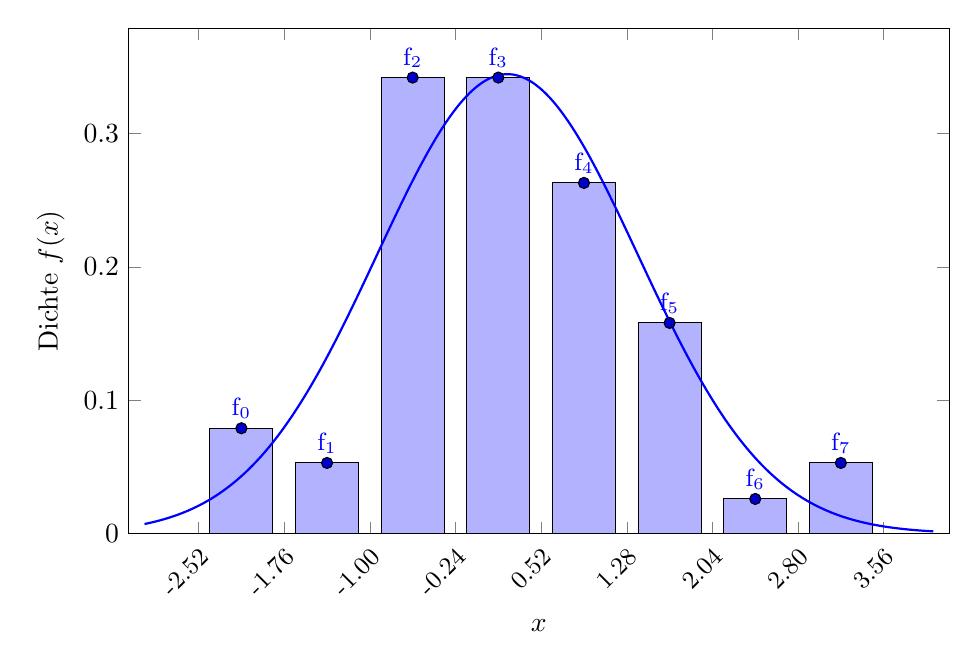
\begin{tikzpicture}
        \pgfmathsetmacro{\mu}{0.221}
        \pgfmathsetmacro{\sigma}{1.158}
        \begin{axis}[
            width=12cm, height=8cm,
            xlabel={$x$}, ylabel={Dichte $f(x)$},
            ymin=0, enlarge x limits=0.02,
            xtick={-2.52,-1.76,-1.00,-0.24,0.52,1.28,2.04,2.80,3.56},
            xticklabels={-2.52,-1.76,-1.00,-0.24,0.52,1.28,2.04,2.80,3.56},
            x tick label style={rotate=45,anchor=north east,font=\small},
            every node near coord/.append style={font=\small, above},
            legend style={at={(0.95,0.95)}, anchor=north east}
        ]
            % Balkendaten (Mittelpunkt, Dichte, Label)
            \addplot+[ybar, bar width=0.8cm, fill=blue!30, draw=black,
                    nodes near coords={\pgfkeysvalueof{/data point/meta}},
                    point meta=explicit symbolic]
            coordinates {
                (-2.14,0.079)[{f$_0$}]
                (-1.38,0.053)[{f$_1$}]
                (-0.62,0.342)[{f$_2$}]
                (0.14,0.342)[{f$_3$}]
                (0.90,0.263)[{f$_4$}]
                (1.66,0.158)[{f$_5$}]
                (2.42,0.026)[{f$_6$}]
                (3.18,0.053)[{f$_7$}]
            };

            % Normalverteilungskurve
            \addplot[domain=-3:4, samples=200, smooth, thick, blue] 
            {1/(\sigma*sqrt(2*pi)) * exp(-((x-\mu)^2)/(2*\sigma^2))};
            %\addlegendentry{Normal($\mu$, $\sigma$)}
        \end{axis}
        \end{tikzpicture}
    \end{center}

    Der Graph scheint grob mit der Dichte Normalverteilung übereinzustimmen, wenn diese die Parameter 
    $\mu=\overline{x}_n$ und $\sigma^2=s_n^2$ hat.
\end{colbox}

\newpage
\subsection*{\underline{Aufgaben:}}

\begin{aufgabe}
Als Lagemaß wird eine Abbildung \(\ell: \mathbb{R}^n \to \mathbb{R}\) bezeichnet, welche für jedes \(c \in \mathbb{R}\) die Bedingung
\[
\ell(x_1 + c, \dots, x_n + c) \;=\; \ell(x_1, \dots, x_n) + c
\]
erfüllt. Als Streuungsmaß hingegen bezeichnen wir eine Abbildung \(s: \mathbb{R}^n \to \mathbb{R}\) mit
\[
s(x_1 + c, \dots, x_n + c) \;=\; s(x_1, \dots, x_n)
\]
für jedes \(c \in \mathbb{R}\). Entscheiden Sie jeweils, ob es sich bei dem Stichprobenmittel und der Stichprobenvarianz um ein Lagemaß oder ein Streuungsmaß handelt.
\end{aufgabe}

\begin{aufgabe}
Seien \(X_1, \dots, X_n\) quadratintegrierbare, unabhängige und identisch verteilte Zufallsvariablen mit Erwartungswert \(\mu\) und Varianz \(\nu\). Wir betrachten für reelle Konstanten \(\alpha_1,\dots,\alpha_n\) die Stichprobenfunktion
\[
\varphi: \mathbb{R}^n \to \mathbb{R},\qquad
\varphi(x_1,\dots,x_n)=\sum_{j=1}^n \alpha_j x_j.
\]
Bestimmen Sie die Koeffizienten \(\alpha_1,\dots,\alpha_n\) derart, dass \(\mathrm{E}[\varphi(X_1,\dots,X_n)]=\mu\) gilt und \(\mathrm{D}^2[\varphi(X_1,\dots,X_n)]\) minimal wird.
\end{aufgabe}

\begin{aufgabe}
\begin{enumerate}
  \item Für die Zufallsvariable \(Y\colon \Omega\to\mathbb{R}\) gelte \(Y\sim \Gamma(b,p)\) mit den Parametern \(b,p>0\), das heißt \(Y\) besitze die Dichte
  \[
    f_Y(y)
    = \frac{b^p}{\Gamma(p)} e^{-b y} y^{p-1} \mathbf{1}_{(0,\infty)}(y).
  \]
  Bestimmen Sie die charakteristische Funktion von \(Y\).
  \item Seien \(Y_1,Y_2\) unabhängige Zufallsvariablen mit \(Y_1\sim \Gamma(b,p_1)\) und \(Y_2\sim \Gamma(b,p_2)\). Zeigen Sie, dass dann \(Y_1+Y_2\sim \Gamma(b,p_1+p_2)\) gilt.
\end{enumerate}
\end{aufgabe}

\begin{aufgabe}
Sei \(r\in\mathbb{N}\) und seien \(X_1,\dots,X_r\) unabhängige und standardnormalverteilte Zufallsvariablen. Zeigen Sie, dass die Zufallsvariable
\[
  U_r = \sum_{i=1}^r X_i^2
\]
chi‑quadratisch mit \(r\) Freiheitsgraden ist, das heißt \(U_r\sim \chi^2_r\) und die Dichte
\[
  f_{U_r}(x)
  = \frac{1}{2^{r/2}\,\Gamma(r/2)}\,x^{\frac{r-2}{2}}e^{-x/2}\,\mathbf{1}_{(0,\infty)}(x)
\]
hat.
\end{aufgabe}

\begin{aufgabe}
Führen Sie zur näherungsweisen Berechnung des Integrals
\[
  \int_{0}^{\frac{\pi}{2}} \sin x \, dx
\]
eine Monte‑Carlo‑Simulation mit Hilfe von MATLAB durch. Nutzen Sie dabei \(n = 10^i\) Samples für \(i \in \{1,\dots,6\}\). Stellen Sie anschließend den absoluten Fehler der numerisch bestimmten Werte von dem korrekten Integralwert in Abhängigkeit von der Anzahl der Samples in einem doppelt‑logarithmischen Diagramm dar.
\end{aufgabe}

\begin{aufgabe}
Gegeben sei eine Stichprobe \((X_1,\dots,X_n)\) von der mit Parameter \(p\in(0,1)\) Bernoulli‑verteilten Zufallsgröße \(X\). Wir wollen nun \(p^2\) mit Hilfe der zufälligen Stichprobenfunktion
\[
  \varphi_1(X_1,\dots,X_n) \;=\; X_1 \cdot X_2
\]
schätzen.
\begin{enumerate}
  \item Bestimmen Sie den Erwartungswert und die Varianz von \(\varphi_1(X_1,\dots,X_n)\). Geben Sie zudem die kleinste Konstante \(c\) an, sodass für alle \(p\in(0,1)\) die Bedingung
  \[
    \mathrm{D}^2\bigl(\varphi_1(X_1,\dots,X_n)\bigr) \;\le\; c
  \]
  erfüllt ist.
  \item Wir definieren eine zweite zufällige Stichprobenfunktion durch
  \[
    \varphi_2(X_1,\dots,X_n)
    = \mathrm{E}\bigl[\varphi_1(X_1,\dots,X_n)\,\bigm|\,S\bigr],
    \quad
    S = \sum_{j=1}^n X_j.
  \]
  Bestimmen Sie den Erwartungswert von \(\varphi_2(X_1,\dots,X_n)\).
  \item Zeigen Sie mit Hilfe der Jensen‑Ungleichung, dass
  \[
    \mathrm{D}^2\bigl[\varphi_1(X_1,\dots,X_n)\bigr]
    \;\ge\;
    \mathrm{D}^2\bigl[\varphi_2(X_1,\dots,X_n)\bigr].
  \]
\end{enumerate}
\end{aufgabe}

\begin{aufgabe}
\begin{enumerate}
  \item Die Stichprobenvariablen \(X_1,\dots,X_n\) seien absolut stetig mit der stückweise stetigen Dichte \(f\colon\mathbb{R}\to[0,\infty)\) und \(X_{(1)},\dots,X_{(n)}\) die zugehörigen Ordnungsstatistiken. Zeigen Sie, dass die gemeinsame Dichte \(f_{X_{(i)},X_{(j)}}\colon\mathbb{R}^2\to[0,\infty)\) für \(1\le i<j\le n\) durch
  \[
    f_{X_{(i)},X_{(j)}}(x_i,x_j)
    =
    \begin{cases}
      \displaystyle
      \frac{n!\,f(x_i)\,f(x_j)\,\bigl(F(x_i)\bigr)^{i-1}\,\bigl(F(x_j)-F(x_i)\bigr)^{\,j-1-i}\,\bigl(1-F(x_j)\bigr)^{\,n-j}}
           {(i-1)!\,(j-1-i)!\,(n-j)!}, 
      & -\infty<x_i<x_j<\infty,\\
      0, & \text{sonst}
    \end{cases}
  \]
  gegeben ist.
  \item Die Stichprobenvariablen \(X_1,\dots,X_n\) seien gleichverteilt im Intervall \((0,b)\) für ein \(b>0\). Bestimmen Sie die Dichte der Spannweite \(R_n = X_{(n)} - X_{(1)}\).
\end{enumerate}
\end{aufgabe}

\begin{aufgabe}
Sei \((X_1,\dots,X_n)\) eine Stichprobe für \(X\), dessen \(k\)-tes Moment existiert. Zeigen Sie, dass
\[
  \hat\mu_k
  = \frac{1}{n-1}
    \sum_{i=1}^n (X_i - X_n)^k
  \quad\text{für }n\to\infty
\]
fast sicher gegen \(\mathrm{E}\bigl[(X - \mathrm{E}[X])^k\bigr]\) konvergiert.
\end{aufgabe}

\begin{aufgabe}
Für zwei Verteilungsfunktionen \(F\) und \(G\) ist der Kolmogorov‑Abstand durch
\[
  d_K(F,G) \;=\; \sup_{x\in\mathbb{R}} \bigl|F(x) - G(x)\bigr|
\]
definiert. Zeigen Sie:
\begin{enumerate}
  \item Der Kolmogorov‑Abstand ist eine Metrik auf dem Raum der Verteilungsfunktionen.
  \item Sei \((X_n)_{n\in\mathbb{N}}\) eine Folge von Zufallsvariablen mit Verteilungsfunktionen \((F_n)\) und \(X\) eine Zufallsvariable mit Verteilungsfunktion \(F\). Zeigen Sie, dass aus
  \[
    d_K(F_n,F)\;\xrightarrow{n\to\infty}\;0
  \]
  die Konvergenz in Verteilung von \((X_n)\) gegen \(X\) folgt, und dass die Umkehrung im Allgemeinen nicht gilt.
\end{enumerate}
\end{aufgabe}

\begin{aufgabe}
Sei \(X_1,\dots,X_n\) eine Stichprobe mit Verteilungsfunktion \(F\). Als Schätzer für \(F\) verwenden wir die empirische Verteilungsfunktion \(W_n\). Zeigen Sie,
\[
  \int_{\mathbb{R}}
  \frac{\bigl|W_n(t) - F(t)\bigr|^2}{1 + t^2}\,dt
  \;\xrightarrow{P}\;0.
\]
\end{aufgabe}

\begin{aufgabe}
Sie führen eine Studie durch, welche den Zusammenhang zwischen Studiendauer und Einstiegsgehalt von Universitätsabsolventen der Wirtschaftswissenschaften untersucht. Das Ergebnis ist in der folgenden Tabelle angegeben:

\begin{center}
\begin{tabular}{r|*{11}{r}}
Absolvent \(i\)              & 1 & 2 & 3 & 4 & 5 & 6 & 7 & 8 & 9 & 10 & 11 \\ \hline
Studiendauer \(x_i\) (Sem.)  & 7 & 10 & 8 & 10 & 6 & 11 & 7 & 8 & 7 & 11 & 12 \\
Einkommen \(y_i\) (\(10^3€\)) & 34 & 58 & 29 & 61 & 40 & 51 & 39 & 64 & 39 & 56 & 59
\end{tabular}
\end{center}

\begin{enumerate}
  \item Berechnen Sie das konkrete Stichprobenmittel und die konkrete Stichprobenvarianz der Stichprobe für \(X\) (Studiendauer) sowie \(Y\) (Einkommen).
  \item Berechnen Sie die Kovarianz sowie den Korrelationskoeffizienten zwischen den beiden Merkmalen. Welche Schlussfolgerung ergibt sich daraus?
  \item Plotten Sie ein Streudiagramm von \((x_i,y_i)\). Bewerten Sie Ihre Schlussfolgerung aus (ii) vor dem Hintergrund des Diagramms.
  \item Markieren Sie im Streudiagramm die Bachelor‑Absolventen (i=1,3,5,7,9) und die Master‑Absolventen (i=2,4,6,8,10,11) unterschiedlich.
  \item Wie ändert sich die Interpretation des Zusammenhangs zwischen Studiendauer und Einstiegsgehalt?
\end{enumerate}
\end{aufgabe}

\begin{aufgabe}
Sei \(X_1,\dots,X_n\) eine Stichprobe mit \(X_1\sim\mathrm{Exp}(1/\theta)\), \(\theta>0\). Gegeben seien die Schätzer
\[
  T_1 = n\cdot \min\{X_1,\dots,X_n\},
  \quad
  T_2 = \frac{1}{n}\sum_{i=1}^n X_i.
\]
\begin{enumerate}
  \item Bestimmen Sie Erwartungswert und Varianz beider Schätzer. Welchen würden Sie bevorzugen und warum?
  \item Entscheiden Sie, ob \(T_1\) in Wahrscheinlichkeit gegen \(\theta\) konvergiert, und begründen Sie Ihre Entscheidung.
\end{enumerate}
\end{aufgabe}

